%%%%%%%%%%%%%%%%%%%%%%%%%%%%%%% SECCIÓN 5 - DOCKER COMPOSE %%%%%%%%%%%%%%%%%%%%%%%%%%%%%%%
\subsection{docker-compose}
\par \texttt{Docker Compose} es una herramienta de \texttt{Docker} 
que sirve para construir, lanzar y gestionar
aplicaciones multicontenedor.

\subsubsection{Instalación}
\par Tengo instalado \texttt{Docker Engine} y \texttt{Docker CLI}, por tanto solo 
hace falta instalar el plugin \texttt{Compose CLI}. Para ello, 
lo descargo e instalo, le aplico permisos de ejecución 
al binario y compruebo que la instalación ha sido un éxito. 
\begin{listing}[style=consola]
    $ DOCKER_CONFIG=${DOCKER_CONFIG:-$HOME/.docker}
    $ mkdir -p $DOCKER_CONFIG/cli-plugins
    $ curl -SL https://github.com/docker/compose/releases/download/v2.6.1/docker-compose-linux-x86_64 -o $DOCKER_CONFIG/cli-plugins/docker-compose
      % Total    % Received % Xferd  Average Speed   Time    Time     Time  Current
      Dload  Upload   Total   Spent    Left  Speed
      0     0    0     0    0     0      0      0 --:--:-- --:--:-- --:--:--     0
    100 24.5M  100 24.5M    0     0  3631k      0  0:00:06  0:00:06 --:--:-- 4177k
    $ chmod +x $DOCKER_CONFIG/cli-plugins/docker-compose
    $ docker compose version
    Docker Compose version v2.6.1
\end{listing}

\subsubsection{Creación del archivo \texttt{.yaml}}
\par En este archivo se definen los contenedores e imágenes
descritos en las secciones anteriores. 
El \texttt{path} por defecto de un archivo \texttt{Compose}
es \texttt{compose.yaml}, por tanto lo crearé con este nombre. Sin embargo,
también soporta \texttt{compose.yml}, \texttt{docker-compose.yaml} y 
\texttt{docker-compose.yml}.

\begin{listing}[style=consola]
    $ touch compose.yaml
\end{listing}

\par \textbf{Version:}
\par El fichero tiene distinto formato dependiendo de la versión
escogida. La definición de la versión está en desuso y solo es informativa. En mi caso selecciono por defecto \texttt{Compose Specification}, porque es la más reciente 
y recomendada, como se indica en la Figura \ref{fig:docker-compose-version} que es definida por \texttt{Compose Specification}
y fusiona las versiones \texttt{2.x} y \texttt{3.x}. Además, es implementada por \texttt{Compose 1.27.0+}.

 %%% IMAGEN DOCKER-COMPOSE VERSION %%%
 \begin{figure}[H]
	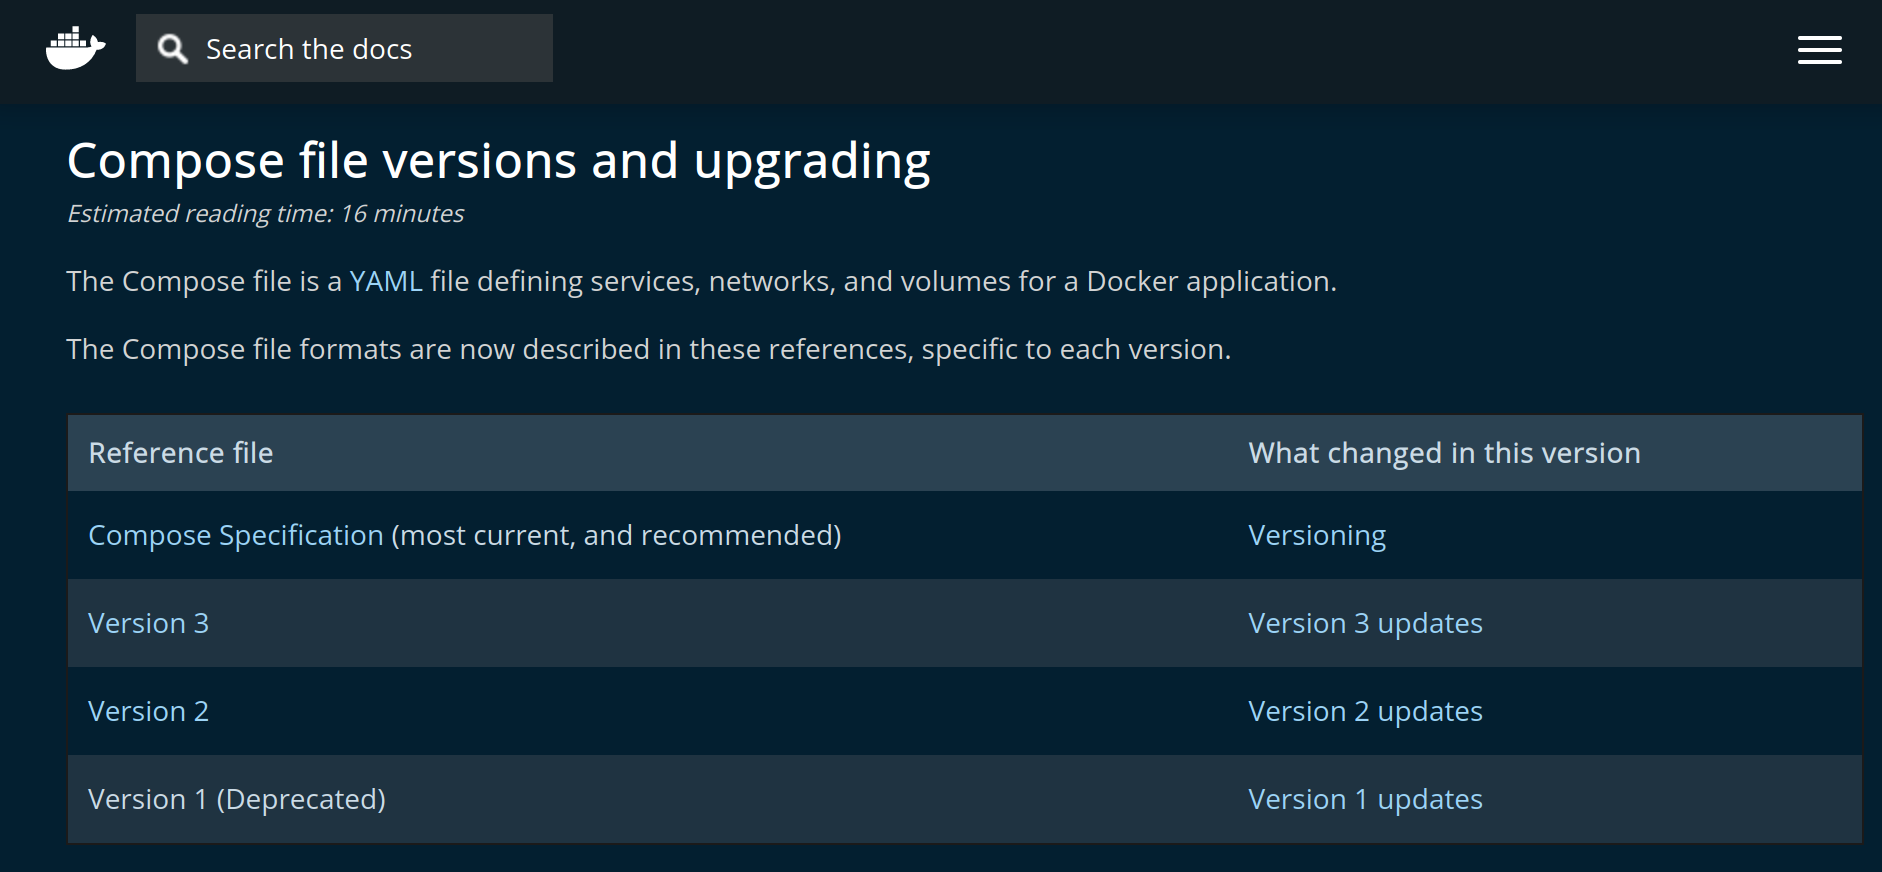
\includegraphics[scale=0.15]{docker-compose-version}
	\centering
	\caption{Versiones del archivo \texttt{Compose}.}
    \label{fig:docker-compose-version}
\end{figure}
\newpage
\par \textbf{Services:}
\par El archivo \texttt{compose.yaml} se compone de servicios.
En está práctica tengo que crear los tres servicios mencionados en las anteriores secciones.
\par Primero, asigno una etiqueta de servicio a cada contenedor
(\texttt{fecha-actual}, \texttt{hora-actual} y \texttt{numero-aleatorio}).
\par Segundo, cada contendor se ejecuta en segundo plano, por tanto, el 
parámetro \texttt{-d} de \texttt{docker run} va implícito.
\par Tercero, puedo definir un nombre a cada contenedor con la etiqueta \texttt{container\_name}.
En este caso, los nombro \texttt{primer-contenedor}, \texttt{segundo-contenedor} y \texttt{tercer-contenedor}.
\par Por último, creo una imagen por cada contenedor y para construirlas busca en el mismo directorio del \texttt{compose.yaml}
el archivo \texttt{Dockerfile} que cada una tiene asignado con un nombre distinto, el mismo que en los anteriores apartados.
\begin{lstlisting}[language=yaml, firstnumber=0]
    @@ +1,20 @@  compose.yaml
    # REQUIRED
    services:
      fecha-actual:
        container_name: primer-contenedor
        image: fecha
        build:
          context: .
          dockerfile: Dockerfile1
      hora-actual:
        container_name: segundo-contenedor
        image: hora
        build:
          context: .
          dockerfile: Dockerfile2
      numero-aleatorio:
        container_name: tercer-contenedor
        image: numero
        build: 
          context: .
          dockerfile: Dockerfile3
\end{lstlisting}

\subsubsection{Construcción de los tres contenedores}
\par El comando \texttt{docker compose build} busca en el directorio actual el archivo
\texttt{compose.yaml} y construye los contenedores y las imágenes de cada servicio descrito 
en ese fichero, como se puede apreciar en la Figura \ref{fig:docker-compose-build}.
%%% IMAGEN DOCKER COMPOSE BUILD %%%
\begin{figure}[H]
    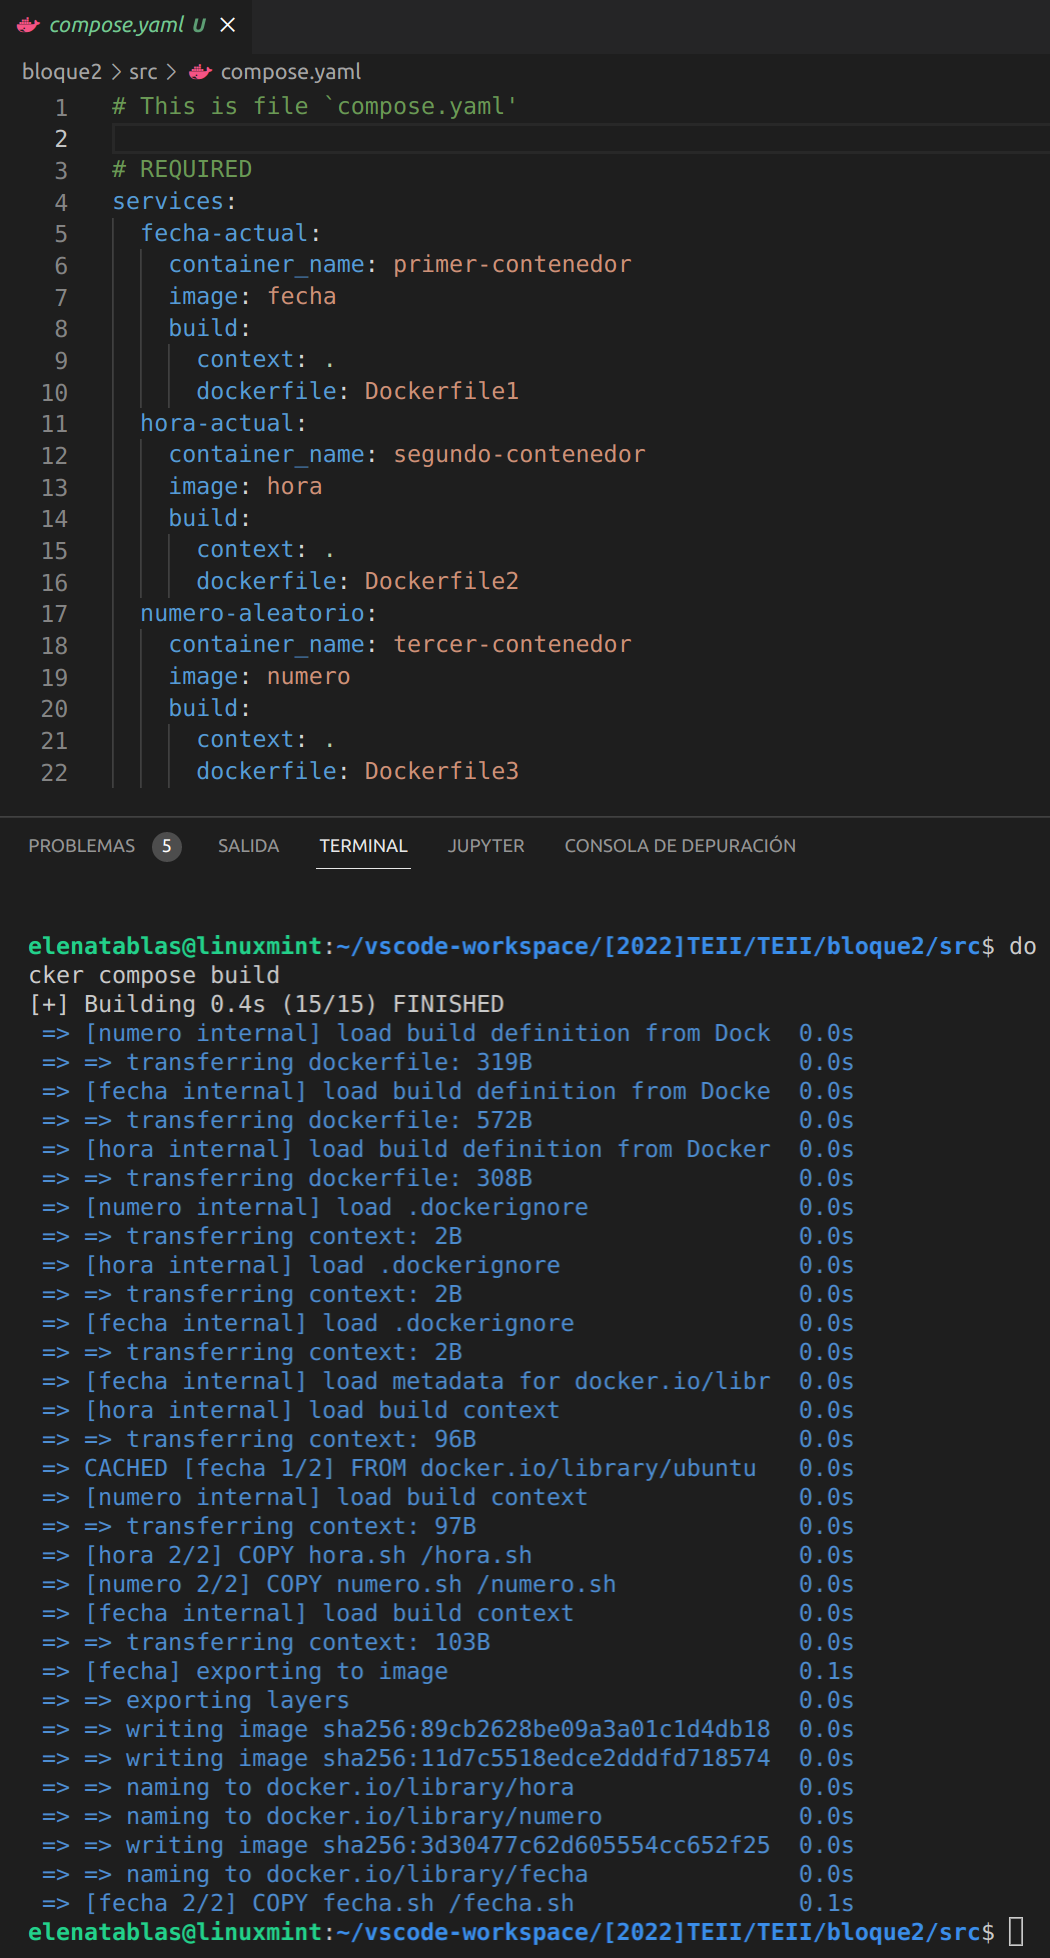
\includegraphics[scale=0.25]{docker-compose-build}
    \centering
    \caption{Construcción de la composición de servicios.}
    \label{fig:docker-compose-build}
 \end{figure}

\subsubsection{Ejecución de los tres contenedores}
\par El comando \texttt{docker compose up}, crea una red donde aloja a los contenedores y 
los ejecuta. Se puede observar como los tres servicios se ejecutan 
a la vez cada segundo tal y como indica el segundo contenedor en la Figura \ref{fig:docker-compose-up}.

%%% IMAGEN DOCKER COMPOSE UP %%%
\begin{figure}[H]
   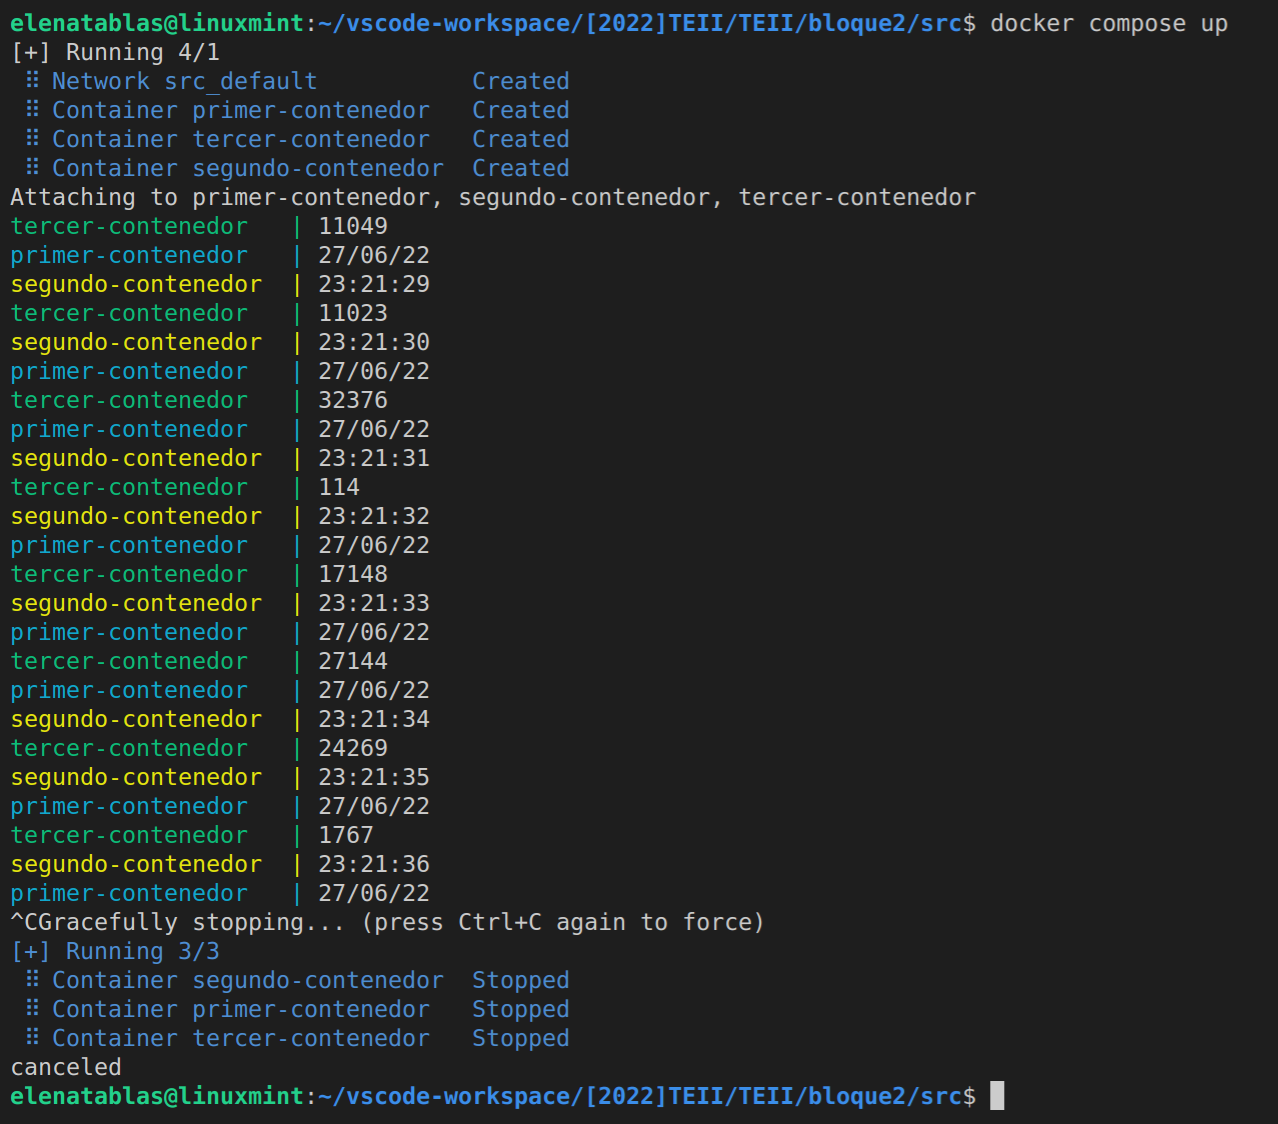
\includegraphics[scale=0.3]{docker-compose-up}
   \centering
   \caption{Ejecución de la composición de servicios.}
   \label{fig:docker-compose-up}
\end{figure}


\subsubsection{Eliminación de los tres contenedores}
\par Utilizo el comando \texttt{docker compose down} para deterner los contenedores y eliminar la red anteriormente
creada por defecto (\texttt{Network src\_default}) junto con los contenedores, como se puede contemplar en la 
Figura \ref{fig:docker-compose-down}.
 %%% IMAGEN DOCKER COMPOSE DOWN %%%
 \begin{figure}[H]
	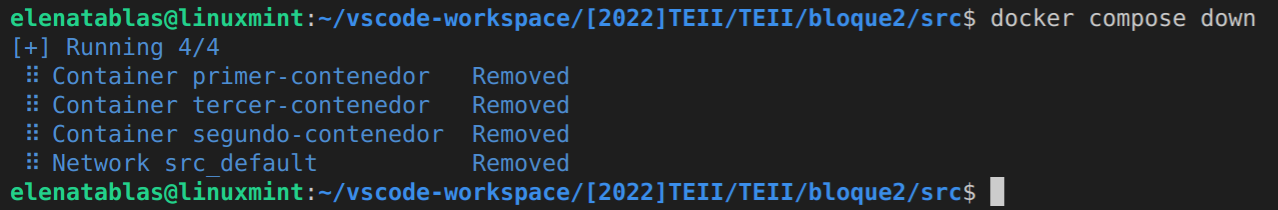
\includegraphics[width=\textwidth]{docker-compose-down}
	\centering
	\caption{Eliminación de la composición de servicios.}
    \label{fig:docker-compose-down}
\end{figure}